\documentclass[12pt]{article} % use larger type; default would be 10pt

\usepackage{pgfplots}
\usetikzlibrary{calc}
\usetikzlibrary{arrows}
\usetikzlibrary{patterns}
\usetikzlibrary{calc,intersections,through,backgrounds}
\usetikzlibrary{decorations.pathreplacing}
        \newcommand\degree[0]{^{\circ}}
        \newcommand\abs[1]{\left|#1\right|}

\title{Play with TikZ}
\author{Just Us}
%\date{} % Activate to display a given date or no date (if empty),
         % otherwise the current date is printed 

\begin{document}
\maketitle

\section{10.2 Polar Graphs }






hp10-2-9ans circles

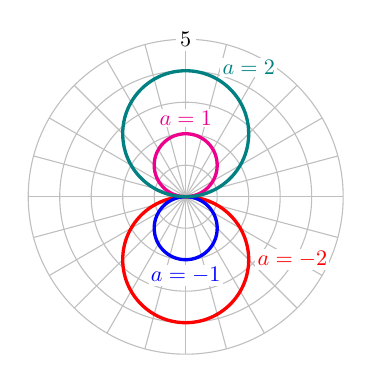
\begin{tikzpicture} [scale=.4]
\coordinate(O) at (0,0);
\foreach \angle [count=\xi] in {0, 15, ..., 345}{
  \draw[lightgray] (\angle:0) -- (\angle:5);
}
\foreach \r in {1,2,3,4,5} {
\draw[lightgray] (O) circle (\r);
}
\node[fill=white, inner sep = 2, text=black, scale=.8] at (90:5) {$5$};
\draw[red,very thick] (0,-2) circle (2cm);
\node[right,fill=white, inner sep=1, scale=.8, text=red] at (2.2,-2)  {$a=-2$};
\draw[blue,very thick] (0,-1) circle (1cm);
\node[fill=white, inner sep=1, scale=.8, text=blue] at (0,-2.5) {$a=-1$};
\draw[magenta,very thick] (0,1) circle (1cm);
\node[fill=white, inner sep=1, scale=.8, text=magenta] at (0,2.5) {$a=1$};
\draw[teal,very thick] (0,2) circle (2cm) ;
\node[fill=white, inner sep=1, scale=.8, text=teal] at (2,4.1) {$a=2$};
\end{tikzpicture}
\newline


hp10-2-11ansa cardioid

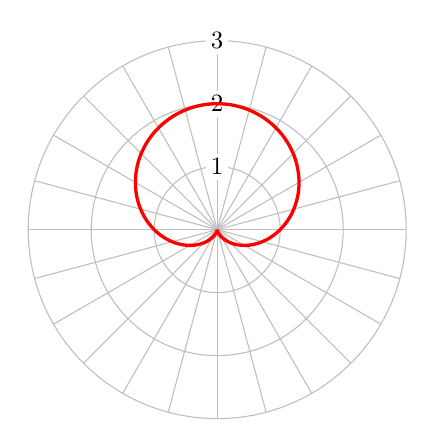
\begin{tikzpicture} [scale=.8]
\coordinate(O) at (0,0);
\foreach \angle [count=\xi] in {0, 15, ..., 345}{
  \draw[lightgray] (\angle:0) -- (\angle:3);
}
\foreach \r in {1,2,3} {
\draw[lightgray] (O) circle (\r);
\node[fill=white, inner sep = 2, text=black, scale=.9] at (90:\r) {$\r$};
}
\draw[domain=0:6,smooth, samples=65,variable=\x,red,very thick] plot ({60*\x)}:{1+sin(60*\x});
\end{tikzpicture}
\newline


hp10-2-11ansb cardioid

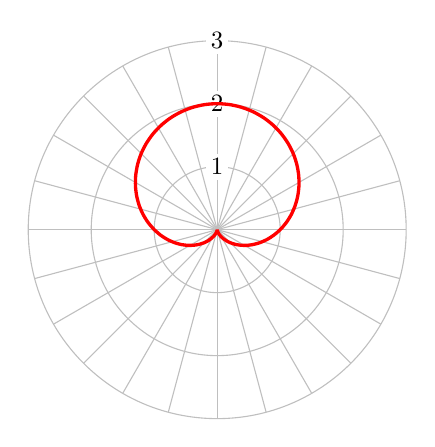
\begin{tikzpicture} [scale=.8]
\coordinate(O) at (0,0);
\foreach \angle [count=\xi] in {0, 15, ..., 345}{
  \draw[lightgray] (\angle:0) -- (\angle:3);
}
\foreach \r in {1,2,3} {
\draw[lightgray] (O) circle (\r);
\node[fill=white, inner sep = 2, text=black, scale=.9] at (90:\r) {$\r$};
}
\draw[domain=0:6,smooth, samples=65,variable=\x,red,very thick] plot ({60*\x)}:{-1+sin(60*\x});
\end{tikzpicture}
\newline


hp10-2-11ansc cardioid

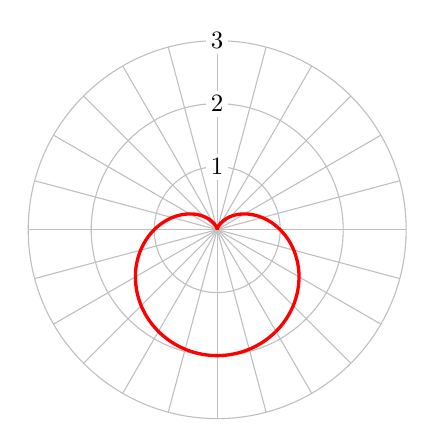
\begin{tikzpicture} [scale=.8]
\coordinate(O) at (0,0);
\foreach \angle [count=\xi] in {0, 15, ..., 345}{
  \draw[lightgray] (\angle:0) -- (\angle:3);
}
\foreach \r in {1,2,3} {
\draw[lightgray] (O) circle (\r);
\node[fill=white, inner sep = 2, text=black, scale=.9] at (90:\r) {$\r$};
}
\draw[domain=0:6,smooth, samples=65,variable=\x,red,very thick] plot ({60*\x)}:{1-sin(60*\x});
\end{tikzpicture}
\newline


hp10-2-11ansd cardioid

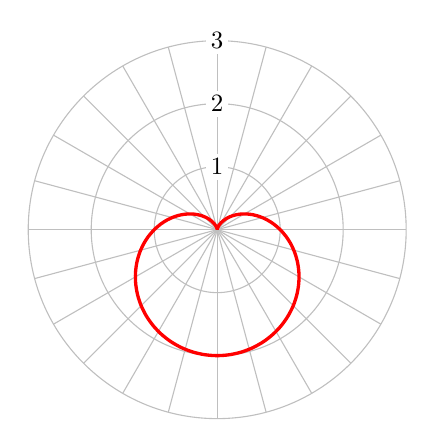
\begin{tikzpicture} [scale=.8]
\coordinate(O) at (0,0);
\foreach \angle [count=\xi] in {0, 15, ..., 345}{
  \draw[lightgray] (\angle:0) -- (\angle:3);
}
\foreach \r in {1,2,3} {
\draw[lightgray] (O) circle (\r);
\node[fill=white, inner sep = 2, text=black, scale=.9] at (90:\r) {$\r$};
}
\draw[domain=0:6,smooth, samples=65,variable=\x,red,very thick] plot ({60*\x)}:{-1-sin(60*\x});
\end{tikzpicture}
\newline


hp10-2-13ansa limacon

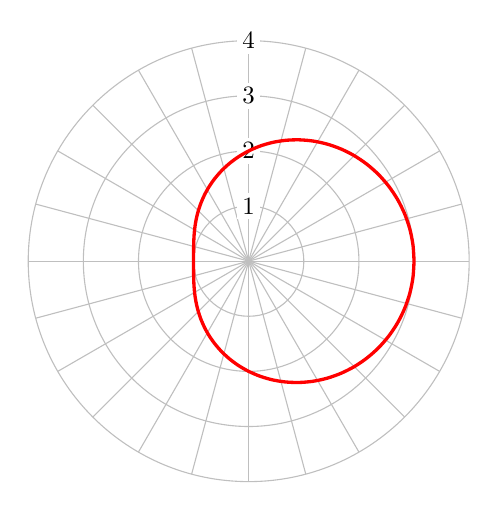
\begin{tikzpicture} [scale=.7]
\coordinate(O) at (0,0);
\foreach \angle [count=\xi] in {0, 15, ..., 345}{
  \draw[lightgray] (\angle:0) -- (\angle:4);
}
\foreach \r in {1,2,3,4} {
\draw[lightgray] (O) circle (\r);
\node[fill=white, inner sep = 2, text=black, scale=.9] at (90:\r) {$\r$};
}
\draw[domain=0:6,smooth, samples=65,variable=\x,red,very thick] plot ({60*\x)}:{2+cos(60*\x});
\end{tikzpicture}
\newline


hp10-2-13ansb limacon

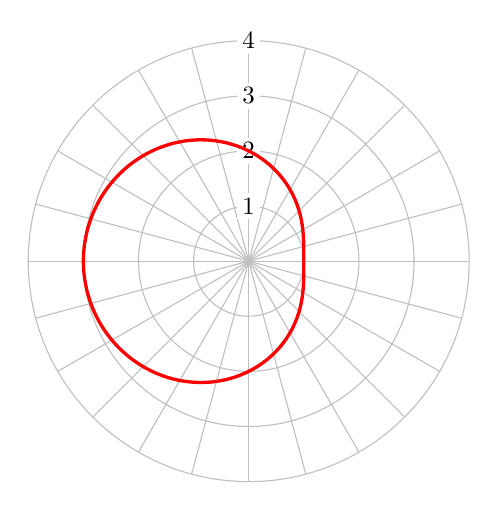
\begin{tikzpicture} [scale=.7]
\coordinate(O) at (0,0);
\foreach \angle [count=\xi] in {0, 15, ..., 345}{
  \draw[lightgray] (\angle:0) -- (\angle:4);
}
\foreach \r in {1,2,3,4} {
\draw[lightgray] (O) circle (\r);
\node[fill=white, inner sep = 2, text=black, scale=.9] at (90:\r) {$\r$};
}
\draw[domain=0:6,smooth, samples=65,variable=\x,red,very thick] plot ({60*\x)}:{2-cos(60*\x});
\end{tikzpicture}
\newline


hp10-2-13ansc limacon

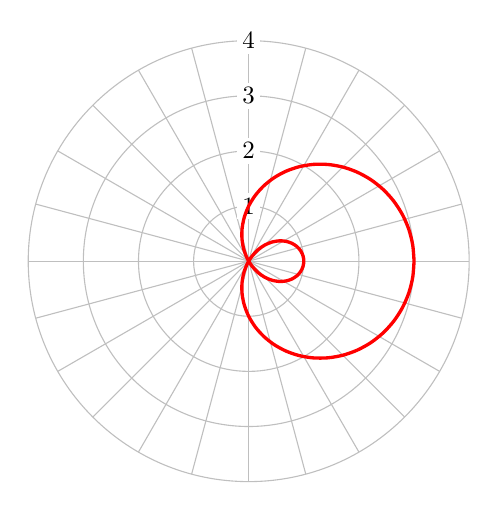
\begin{tikzpicture} [scale=.7]
\coordinate(O) at (0,0);
\foreach \angle [count=\xi] in {0, 15, ..., 345}{
  \draw[lightgray] (\angle:0) -- (\angle:4);
}
\foreach \r in {1,2,3,4} {
\draw[lightgray] (O) circle (\r);
\node[fill=white, inner sep = 2, text=black, scale=.9] at (90:\r) {$\r$};
}
\draw[domain=0:6,smooth, samples=65,variable=\x,red,very thick] plot ({60*\x)}:{1+2*cos(60*\x});
\end{tikzpicture}
\newline


hp10-2-13ansd limacon

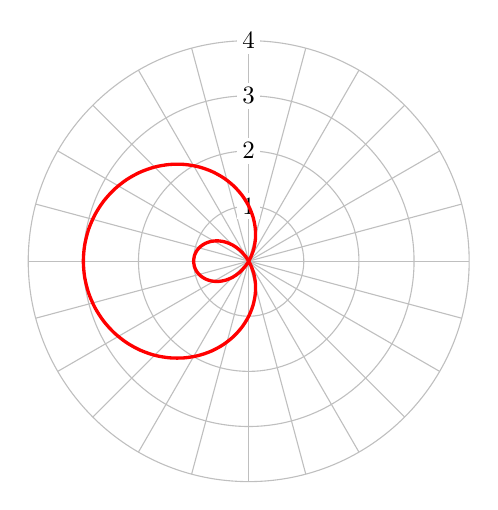
\begin{tikzpicture} [scale=.7]
\coordinate(O) at (0,0);
\foreach \angle [count=\xi] in {0, 15, ..., 345}{
  \draw[lightgray] (\angle:0) -- (\angle:4);
}
\foreach \r in {1,2,3,4} {
\draw[lightgray] (O) circle (\r);
\node[fill=white, inner sep = 2, text=black, scale=.9] at (90:\r) {$\r$};
}
\draw[domain=0:6,smooth, samples=65,variable=\x,red,very thick] plot ({60*\x)}:{1-2*cos(60*\x});
\end{tikzpicture}
\newline



hp10-2-15ansa1 4-petal rose

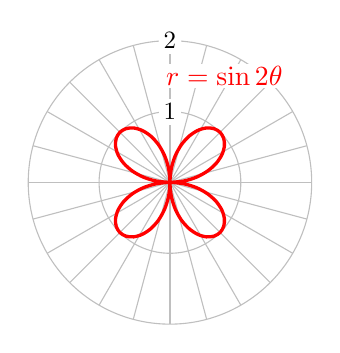
\begin{tikzpicture} [scale=.9]
\coordinate(O) at (0,0);
\foreach \angle [count=\xi] in {0, 15, ..., 345}{
  \draw[lightgray] (\angle:0) -- (\angle:2);
}
\foreach \r in {1,2} {
\draw[lightgray] (O) circle (\r);
\node[fill=white, inner sep = 2, text=black, scale=.9] at (90:\r) {$\r$};
}
\draw[domain=0:6,smooth, samples=65,variable=\x,red,very thick] plot ({60*\x)}:{sin(2*60*\x});
\node[right,text=red, fill=white, inner sep =1] at (-.1,1.5) {$r=\sin 2\theta$};
\end{tikzpicture}
\newline



hp10-2-15ansa2 3-petal rose

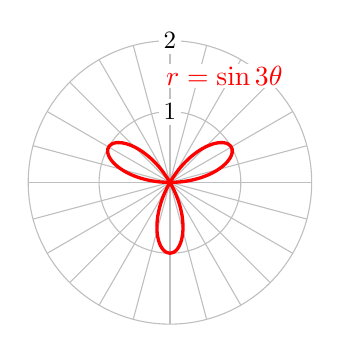
\begin{tikzpicture} [scale=.9]
\coordinate(O) at (0,0);
\foreach \angle [count=\xi] in {0, 15, ..., 345}{
  \draw[lightgray] (\angle:0) -- (\angle:2);
}
\foreach \r in {1,2} {
\draw[lightgray] (O) circle (\r);
\node[fill=white, inner sep = 2, text=black, scale=.9] at (90:\r) {$\r$};
}
\draw[domain=0:3,smooth, samples=65,variable=\x,red,very thick] plot ({60*\x)}:{sin(3*60*\x});
\node[right,text=red, fill=white, inner sep =1] at (-.1,1.5) {$r=\sin 3\theta$};
\end{tikzpicture}
\newline



hp10-2-15ansa3 8-petal rose

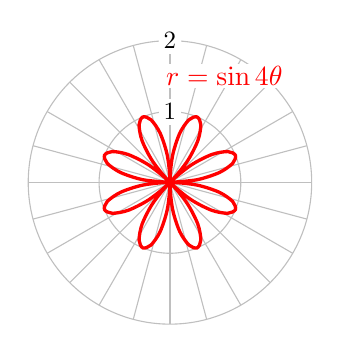
\begin{tikzpicture} [scale=.9]
\coordinate(O) at (0,0);
\foreach \angle [count=\xi] in {0, 15, ..., 345}{
  \draw[lightgray] (\angle:0) -- (\angle:2);
}
\foreach \r in {1,2} {
\draw[lightgray] (O) circle (\r);
\node[fill=white, inner sep = 2, text=black, scale=.9] at (90:\r) {$\r$};
}
\draw[domain=0:6,smooth, samples=65,variable=\x,red,very thick] plot ({60*\x)}:{sin(4*60*\x});
\node[right,text=red, fill=white, inner sep =1] at (-.1,1.5) {$r=\sin 4\theta$};
\end{tikzpicture}
\newline



hp10-2-15ansa4 5-petal rose

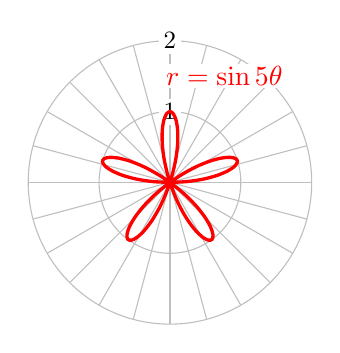
\begin{tikzpicture} [scale=.9]
\coordinate(O) at (0,0);
\foreach \angle [count=\xi] in {0, 15, ..., 345}{
  \draw[lightgray] (\angle:0) -- (\angle:2);
}
\foreach \r in {1,2} {
\draw[lightgray] (O) circle (\r);
\node[fill=white, inner sep = 2, text=black, scale=.9] at (90:\r) {$\r$};
}
\draw[domain=0:3,smooth, samples=65,variable=\x,red,very thick] plot ({60*\x)}:{sin(5*60*\x});
\node[right,text=red, fill=white, inner sep =1] at (-.1,1.5) {$r=\sin 5\theta$};
\end{tikzpicture}
\newline



hp10-2-15ansc1 3-petal rose

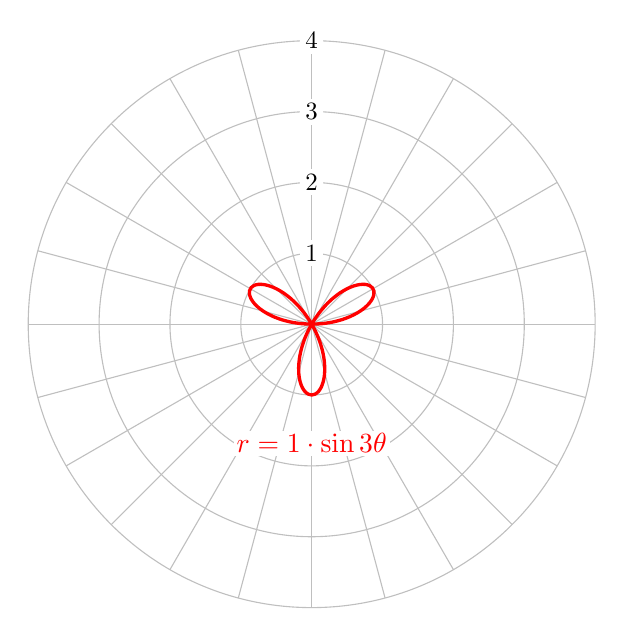
\begin{tikzpicture} [scale=.9]
\coordinate(O) at (0,0);
\foreach \angle [count=\xi] in {0, 15, ..., 345}{
  \draw[lightgray] (\angle:0) -- (\angle:4);
}
\foreach \r in {1,2,3,4} {
\draw[lightgray] (O) circle (\r);
\node[fill=white, inner sep = 2, text=black, scale=.9] at (90:\r) {$\r$};
}
\draw[domain=0:3,smooth, samples=65,variable=\x,red,very thick] plot ({60*\x)}:{sin(3*60*\x});
\node[below,text=red, fill=white, inner sep =1] at (0,-1.5) {$r=1\cdot\sin 3\theta$};
\end{tikzpicture}
\newline



hp10-2-15ansc2 3-petal rose

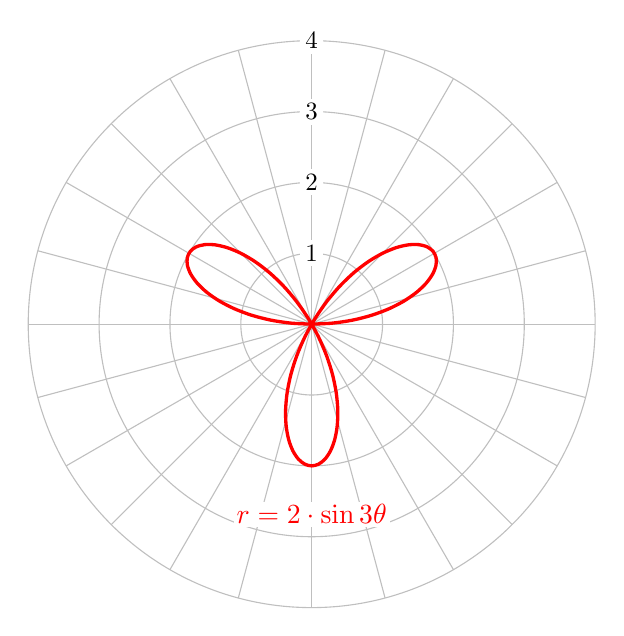
\begin{tikzpicture} [scale=.9]
\coordinate(O) at (0,0);
\foreach \angle [count=\xi] in {0, 15, ..., 345}{
  \draw[lightgray] (\angle:0) -- (\angle:4);
}
\foreach \r in {1,2,3,4} {
\draw[lightgray] (O) circle (\r);
\node[fill=white, inner sep = 2, text=black, scale=.9] at (90:\r) {$\r$};
}
\draw[domain=0:3,smooth, samples=65,variable=\x,red,very thick] plot ({60*\x)}:{2*sin(3*60*\x});
\node[below,text=red, fill=white, inner sep =1] at (0,-2.5) {$r=2\cdot\sin 3\theta$};
\end{tikzpicture}
\newline



hp10-2-15ansc3 3-petal rose

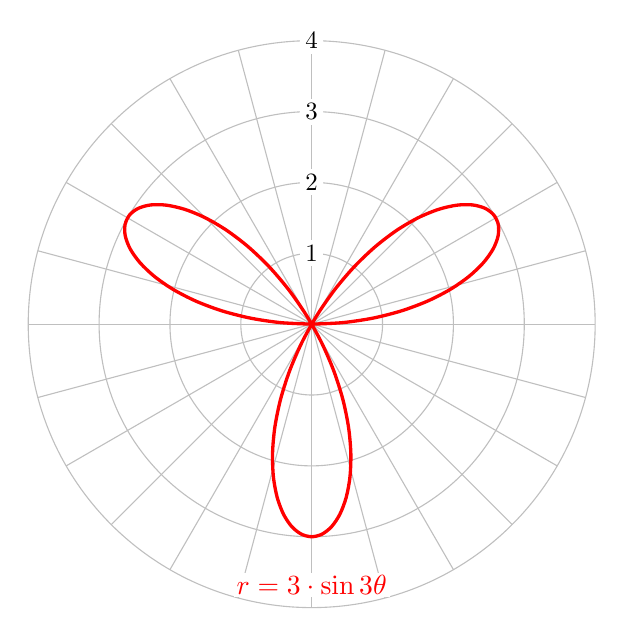
\begin{tikzpicture} [scale=.9]
\coordinate(O) at (0,0);
\foreach \angle [count=\xi] in {0, 15, ..., 345}{
  \draw[lightgray] (\angle:0) -- (\angle:4);
}
\foreach \r in {1,2,3,4} {
\draw[lightgray] (O) circle (\r);
\node[fill=white, inner sep = 2, text=black, scale=.9] at (90:\r) {$\r$};
}
\draw[domain=0:3,smooth, samples=65,variable=\x,red,very thick] plot ({60*\x)}:{3*sin(3*60*\x});
\node[below,text=red, fill=white, inner sep =1] at (0,-3.5) {$r=3\cdot\sin 3\theta$};
\end{tikzpicture}
\newline



hp10-2-17ans leminiscate

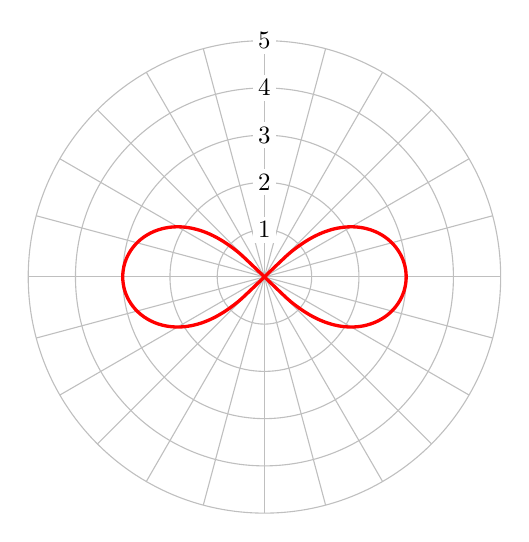
\begin{tikzpicture} [scale=.6]
\coordinate(O) at (0,0);
\foreach \angle [count=\xi] in {0, 15, ..., 345}{
  \draw[lightgray] (\angle:0) -- (\angle:5);
}
\foreach \r in {1,2,3,4,5} {
\draw[lightgray] (O) circle (\r);
\node[fill=white, inner sep = 2, text=black, scale=.9] at (90:\r) {$\r$};
}
\draw[domain=-3:3,smooth, samples=65,variable=\x,red,very thick] plot ({15*\x}:{3*sqrt(cos(30*\x)});
\draw[domain=-3:3,smooth, samples=65,variable=\x,red,very thick] plot ({15*\x}:{-3*sqrt(cos(30*\x)});
\end{tikzpicture}
\newline



hp10-2-19ans Archimedean spiral

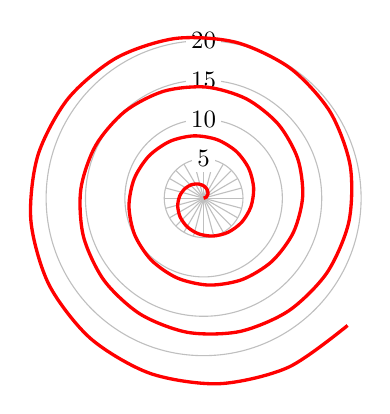
\begin{tikzpicture} [scale=.1]
\coordinate(O) at (0,0);
\foreach \angle [count=\xi] in {0, 15, ..., 345}{
  \draw[lightgray] (\angle:0) -- (\angle:5);
}
\foreach \r in {5,10,15,20} {
\draw[lightgray] (O) circle (\r);
\node[fill=white, inner sep = 2, text=black, scale=.9] at (90:\r) {$\r$};
}
\draw[domain=0:7.77,smooth, samples=65,variable=\x,red,very thick] plot ({180*\x}:{pi*\x)});
\end{tikzpicture}
\newline

hp10-2-21ansa sine graph sin 3theta

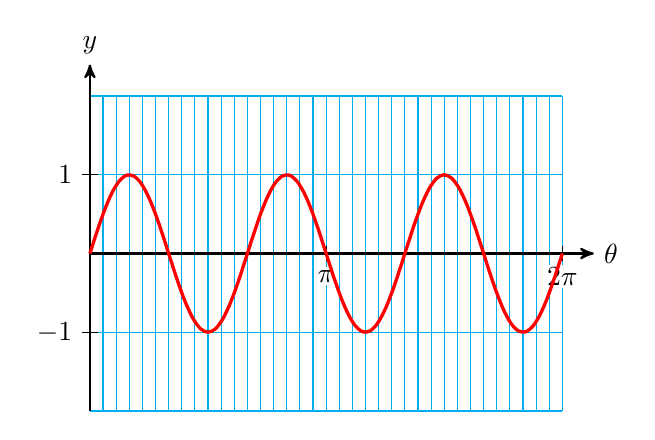
\begin{tikzpicture}
\draw[cyan] (0,-2) grid[xstep=1/6] (6,2);
\draw[black,thick,->,>=stealth'] (0,0)--(6.4,0) node[right]{$\theta$};
\draw[black,thick,->,>=stealth'] (0,-2)--(0, 2.4) node[above]{$y$};
\foreach \y in {-1,1} {
\draw[black] (.1,\y) --++ (-.2,0) node[left]{$\y$};
}
\draw[black] (3,.1) --++ (0,-.2) node[below, yshift=-2, fill=white, inner sep=1]{$\pi$};
\draw[black] (6,.1) --++ (0,-.2) node[below, yshift=-1, fill=white, inner sep=1]{$2\pi$};
\draw[domain=0:6,smooth, samples=65,variable=\x,red,very thick] plot (\x,{sin(180*\x)});

\end{tikzpicture}
\newline


hp10-2-21ansb 3-petal rose

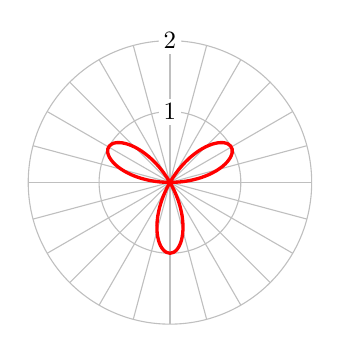
\begin{tikzpicture} [scale=.9]
\coordinate(O) at (0,0);
\foreach \angle [count=\xi] in {0, 15, ..., 345}{
  \draw[lightgray] (\angle:0) -- (\angle:2);
}
\foreach \r in {1,2} {
\draw[lightgray] (O) circle (\r);
\node[fill=white, inner sep = 2, text=black, scale=.9] at (90:\r) {$\r$};
}
\draw[domain=0:3,smooth, samples=65,variable=\x,red,very thick] plot ({60*\x)}:{sin(3*60*\x});
\end{tikzpicture}
\newline

hp10-2-23ansa 2+2 cos theta

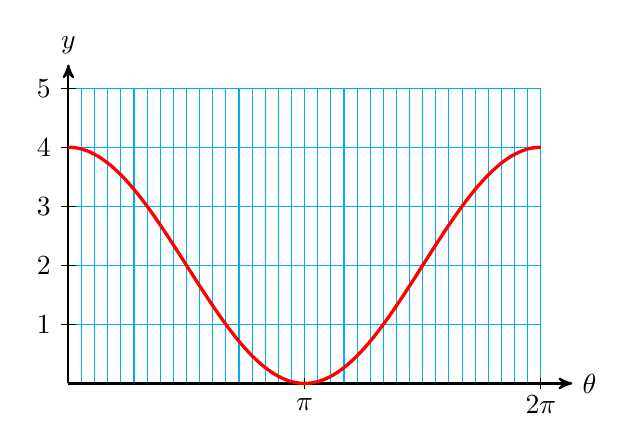
\begin{tikzpicture} [xscale=1, yscale = .75]
\draw[cyan] (0,0) grid[xstep=1/6] (6,5);
\draw[black,thick,->,>=stealth'] (0,0)--(6.4,0) node[right]{$\theta$};
\draw[black,thick,->,>=stealth'] (0,0)--(0, 5.4) node[above]{$y$};
\foreach \y in {1,2,3,4,5} {
\draw[black] (.1,\y) --++ (-.2,0) node[left]{$\y$};
}
\draw[black] (3,.1) --++ (0,-.2) node[below, yshift=-2, fill=white, inner sep=1]{$\pi$};
\draw[black] (6,.1) --++ (0,-.2) node[below, yshift=-1, fill=white, inner sep=1]{$2\pi$};
\draw[domain=0:6,smooth, samples=65,variable=\x,red,very thick] plot (\x,{2+2*cos(60*\x)});

\end{tikzpicture}
\newline


hp10-2-23ansb cardioid

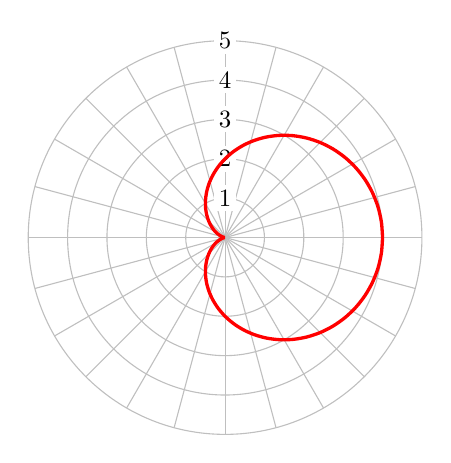
\begin{tikzpicture} [scale=.5]
\coordinate(O) at (0,0);
\foreach \angle [count=\xi] in {0, 15, ..., 345}{
  \draw[lightgray] (\angle:0) -- (\angle:5);
}
\foreach \r in {1,2,3,4,5} {
\draw[lightgray] (O) circle (\r);
\node[fill=white, inner sep = 2, text=black, scale=.9] at (90:\r) {$\r$};
}
\draw[domain=0:2,smooth, samples=65,variable=\x,red,very thick] plot ({180*\x)}:{2+2*cos(180*\x});
\end{tikzpicture}
\newline


hp10-2-25ans circle

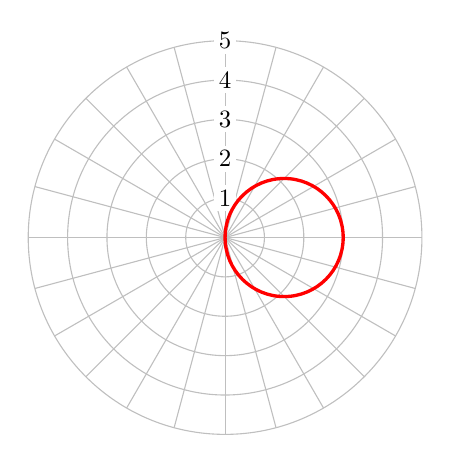
\begin{tikzpicture} [scale=.5]
\coordinate(O) at (0,0);
\foreach \angle [count=\xi] in {0, 15, ..., 345}{
  \draw[lightgray] (\angle:0) -- (\angle:5);
}
\foreach \r in {1,2,3,4,5} {
\draw[lightgray] (O) circle (\r);
\node[fill=white, inner sep = 2, text=black, scale=.9] at (90:\r) {$\r$};
}
\draw[red,very thick] (1.5,0) circle (1.5cm);
\end{tikzpicture}
\newline


hp10-2-27ans 3-line

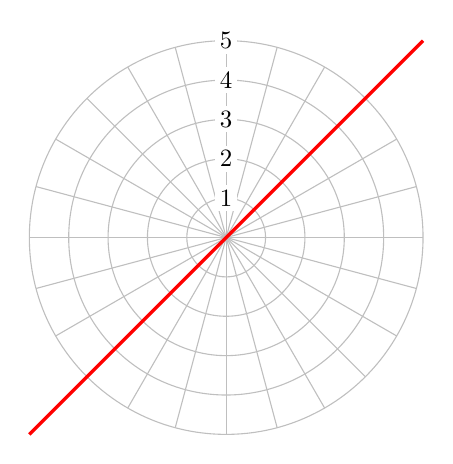
\begin{tikzpicture} [scale=.5]
\coordinate(O) at (0,0);
\foreach \angle [count=\xi] in {0, 15, ..., 345}{
  \draw[lightgray] (\angle:0) -- (\angle:5);
}
\foreach \r in {1,2,3,4,5} {
\draw[lightgray] (O) circle (\r);
\node[fill=white, inner sep = 2, text=black, scale=.9] at (90:\r) {$\r$};
}
\draw[red,very thick] (-5,-5) -- (5,5);
\end{tikzpicture}
\newline


hp10-2-29ans circle

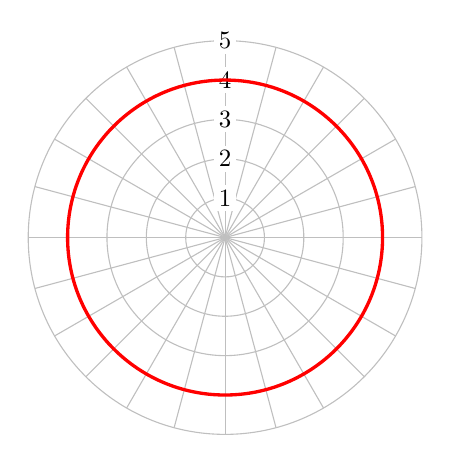
\begin{tikzpicture} [scale=.5]
\coordinate(O) at (0,0);
\foreach \angle [count=\xi] in {0, 15, ..., 345}{
  \draw[lightgray] (\angle:0) -- (\angle:5);
}
\foreach \r in {1,2,3,4,5} {
\draw[lightgray] (O) circle (\r);
\node[fill=white, inner sep = 2, text=black, scale=.9] at (90:\r) {$\r$};
}
\draw[red,very thick] (0,0) circle (4cm);
\end{tikzpicture}
\newline


hp10-2-31ans cardioid

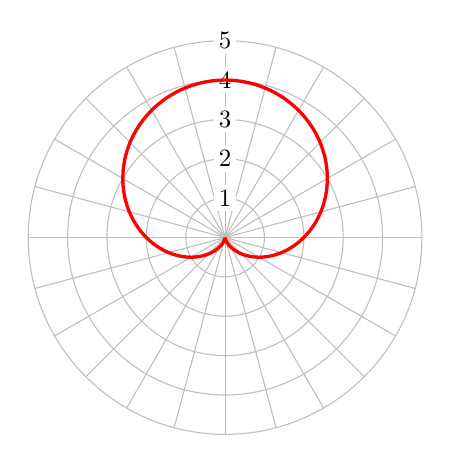
\begin{tikzpicture} [scale=.5]
\coordinate(O) at (0,0);
\foreach \angle [count=\xi] in {0, 15, ..., 345}{
  \draw[lightgray] (\angle:0) -- (\angle:5);
}
\foreach \r in {1,2,3,4,5} {
\draw[lightgray] (O) circle (\r);
\node[fill=white, inner sep = 2, text=black, scale=.9] at (90:\r) {$\r$};
}
\draw[domain=0:2,smooth, samples=65,variable=\x,red,very thick] plot ({180*\x)}:{2+2*sin(180*\x});
\end{tikzpicture}
\newline


hp10-2-33ans limacon

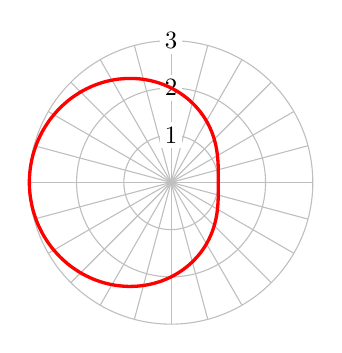
\begin{tikzpicture} [scale=.6]
\coordinate(O) at (0,0);
\foreach \angle [count=\xi] in {0, 15, ..., 345}{
  \draw[lightgray] (\angle:0) -- (\angle:3);
}
\foreach \r in {1,2,3} {
\draw[lightgray] (O) circle (\r);
\node[fill=white, inner sep = 2, text=black, scale=.9] at (90:\r) {$\r$};
}
\draw[domain=0:2,smooth, samples=65,variable=\x,red,very thick] plot ({180*\x)}:{2-cos(180*\x});
\end{tikzpicture}
\newline


hp10-2-35ans four-petal rose

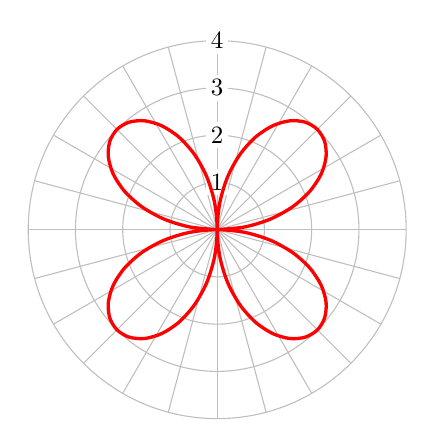
\begin{tikzpicture} [scale=.6]
\coordinate(O) at (0,0);
\foreach \angle [count=\xi] in {0, 15, ..., 345}{
  \draw[lightgray] (\angle:0) -- (\angle:4);
}
\foreach \r in {1,2,3,4} {
\draw[lightgray] (O) circle (\r);
\node[fill=white, inner sep = 2, text=black, scale=.9] at (90:\r) {$\r$};
}
\draw[domain=0:2,smooth, samples=65,variable=\x,red,very thick] plot ({180*\x)}:{3*sin(360*\x});
\end{tikzpicture}
\newline


hp10-2-37ans five-petal rose

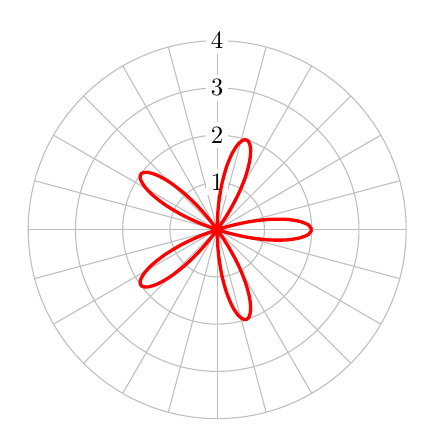
\begin{tikzpicture} [scale=.6]
\coordinate(O) at (0,0);
\foreach \angle [count=\xi] in {0, 15, ..., 345}{
  \draw[lightgray] (\angle:0) -- (\angle:4);
}
\foreach \r in {1,2,3,4} {
\draw[lightgray] (O) circle (\r);
\node[fill=white, inner sep = 2, text=black, scale=.9] at (90:\r) {$\r$};
}
\draw[domain=0:1,smooth, samples=65,variable=\x,red,very thick] plot ({180*\x)}:{2*cos(900*\x});
\end{tikzpicture}
\newline


hp10-2-39ans limacon

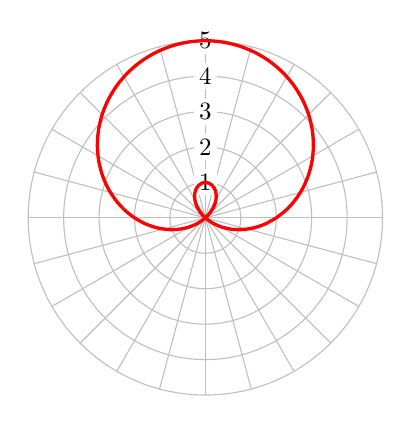
\begin{tikzpicture} [scale=.45]
\coordinate(O) at (0,0);
\foreach \angle [count=\xi] in {0, 15, ..., 345}{
  \draw[lightgray] (\angle:0) -- (\angle:5);
}
\foreach \r in {1,2,3,4,5} {
\draw[lightgray] (O) circle (\r);
\node[fill=white, inner sep = 2, text=black, scale=.9] at (90:\r) {$\r$};
}
\draw[domain=0:2,smooth, samples=65,variable=\x,red,very thick] plot ({180*\x)}:{2+3*sin(180*\x});
\end{tikzpicture}
\newline



hp10-2-41ans leminiscate

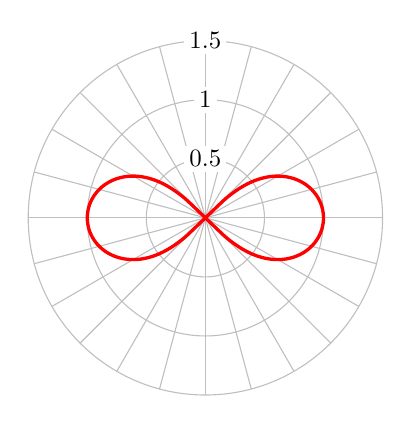
\begin{tikzpicture} [scale=1.5]
\coordinate(O) at (0,0);
\foreach \angle [count=\xi] in {0, 15, ..., 345}{
  \draw[lightgray] (\angle:0) -- (\angle:1.5);
}
\foreach \r in {0.5,1,1.5} {
\draw[lightgray] (O) circle (\r);
\node[fill=white, inner sep = 2, text=black, scale=.9] at (90:\r) {$\r$};
}
\draw[domain=-3:3,smooth, samples=65,variable=\x,red,very thick] plot ({15*\x}:{1*sqrt(cos(30*\x)});
\draw[domain=-3:3,smooth, samples=65,variable=\x,red,very thick] plot ({15*\x}:{-1*sqrt(cos(30*\x)});
\end{tikzpicture}
\newline


hp10-2-43ans circle

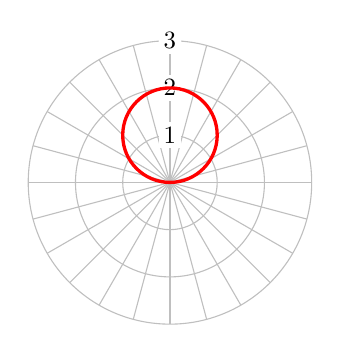
\begin{tikzpicture} [scale=.6]
\coordinate(O) at (0,0);
\foreach \angle [count=\xi] in {0, 15, ..., 345}{
  \draw[lightgray] (\angle:0) -- (\angle:3);
}
\foreach \r in {1,2,3} {
\draw[lightgray] (O) circle (\r);
\node[fill=white, inner sep = 2, text=black, scale=.9] at (90:\r) {$\r$};
}
\draw[red,very thick] (0,1) circle (1cm);
\end{tikzpicture}
\newline


hp10-2-45ans arcs of a circle

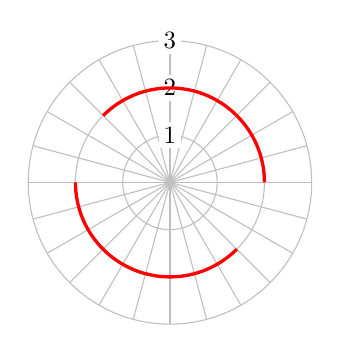
\begin{tikzpicture} [scale=.6]
\coordinate(O) at (0,0);
\foreach \angle [count=\xi] in {0, 15, ..., 345}{
  \draw[lightgray] (\angle:0) -- (\angle:3);
}
\foreach \r in {1,2,3} {
\draw[lightgray] (O) circle (\r);
\node[fill=white, inner sep = 2, text=black, scale=.9] at (90:\r) {$\r$};
}
\draw[red,very thick] (0:2) arc (0:135:2);
\draw[red,very thick] (180:2) arc (180:315:2);
\end{tikzpicture}
\newline



hp10-2-47ans semicircle

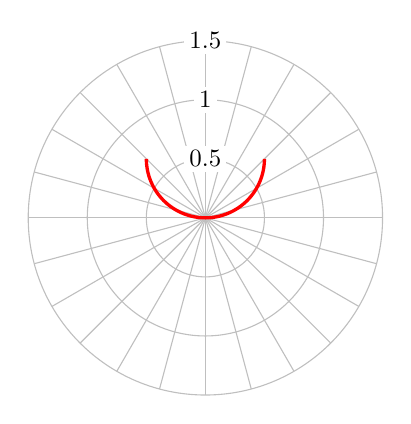
\begin{tikzpicture} [scale=1.5]
\coordinate(O) at (0,0);
\foreach \angle [count=\xi] in {0, 15, ..., 345}{
  \draw[lightgray] (\angle:0) -- (\angle:1.5);
}
\foreach \r in {0.5,1,1.5} {
\draw[lightgray] (O) circle (\r);
\node[fill=white, inner sep = 2, text=black, scale=.9] at (90:\r) {$\r$};
}
\draw[domain=3:5,smooth, samples=65,variable=\x,red,very thick] plot ({45*\x}:{sin(45*\x)});
\end{tikzpicture}
\newline



hp10-2-49ans 8 petal rose

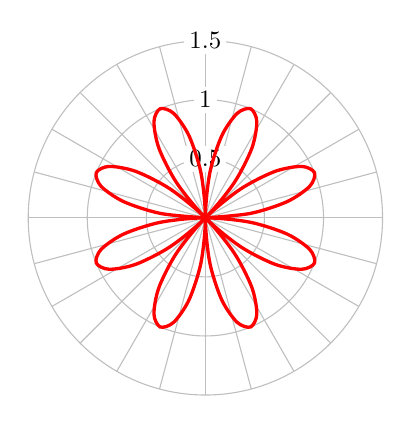
\begin{tikzpicture} [scale=1.5]
\coordinate(O) at (0,0);
\foreach \angle [count=\xi] in {0, 15, ..., 345}{
  \draw[lightgray] (\angle:0) -- (\angle:1.5);
}
\foreach \r in {0.5,1,1.5} {
\draw[lightgray] (O) circle (\r);
\node[fill=white, inner sep = 2, text=black, scale=.9] at (90:\r) {$\r$};
}
\draw[domain=0:2,smooth, samples=65,variable=\x,red,very thick] plot ({180*\x}:{2*sin(2*180*\x)*cos(2*180*\x)});
\end{tikzpicture}
\newline



hp10-2-51ans cardioid

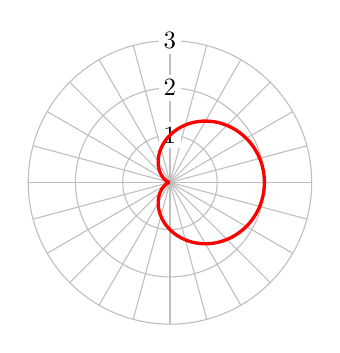
\begin{tikzpicture} [scale=0.6]
\coordinate(O) at (0,0);
\foreach \angle [count=\xi] in {0, 15, ..., 345}{
  \draw[lightgray] (\angle:0) -- (\angle:3);
}
\foreach \r in {1,2,3} {
\draw[lightgray] (O) circle (\r);
\node[fill=white, inner sep = 2, text=black, scale=.9] at (90:\r) {$\r$};
}
\draw[domain=0:2,smooth, samples=65,variable=\x,red,very thick] plot ({180*\x}:{1+cos(180*\x)});
\end{tikzpicture}
\newline



hp10-2-53ans parabola

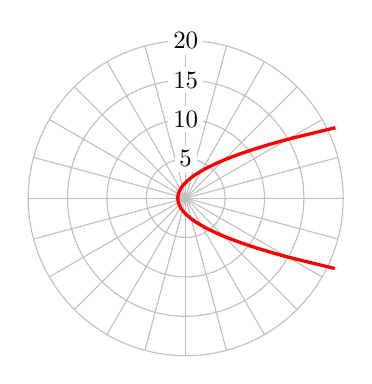
\begin{tikzpicture} [scale=0.1]
\coordinate(O) at (0,0);
\foreach \angle [count=\xi] in {0, 15, ..., 345}{
  \draw[lightgray] (\angle:0) -- (\angle:20);
}
\foreach \r in {5,10,15,20} {
\draw[lightgray] (O) circle (\r);
\node[fill=white, inner sep = 2, text=black, scale=.9] at (90:\r) {$\r$};
}
\draw[domain=.14:1.86,smooth, samples=65,variable=\x,red,very thick] plot ({180*\x}:{2/(1-cos(180*\x))});
\end{tikzpicture}
\newline



hp10-2-55ans ellipse

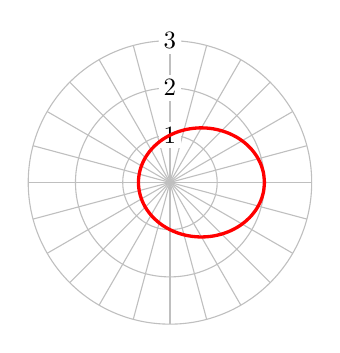
\begin{tikzpicture} [scale=0.6]
\coordinate(O) at (0,0);
\foreach \angle [count=\xi] in {0, 15, ..., 345}{
  \draw[lightgray] (\angle:0) -- (\angle:3);
}
\foreach \r in {1,2,3} {
\draw[lightgray] (O) circle (\r);
\node[fill=white, inner sep = 2, text=black, scale=.9] at (90:\r) {$\r$};
}
\draw[domain=0:2,smooth, samples=65,variable=\x,red,very thick] plot ({180*\x}:{2/(2-cos(180*\x))});
\end{tikzpicture}
\newline



hp10-2-57ans hyperbola

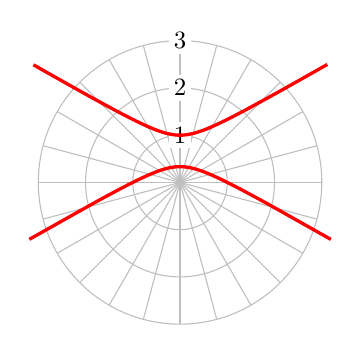
\begin{tikzpicture} [scale=0.6]
\coordinate(O) at (0,0);
\foreach \angle [count=\xi] in {0, 15, ..., 345}{
  \draw[lightgray] (\angle:0) -- (\angle:3);
}
\foreach \r in {1,2,3} {
\draw[lightgray] (O) circle (\r);
\node[fill=white, inner sep = 2, text=black, scale=.9] at (90:\r) {$\r$};
}
\draw[domain=-.115:1.115,smooth, samples=33,variable=\x,red,very thick] plot ({180*\x}:{1/(1+2*sin(180*\x))});
\draw[domain=1.215:1.785,smooth, samples=33,variable=\x,red,very thick] plot ({180*\x}:{1/(1+2*sin(180*\x))});
\end{tikzpicture}
\newline


hp10-2-59 cardioid

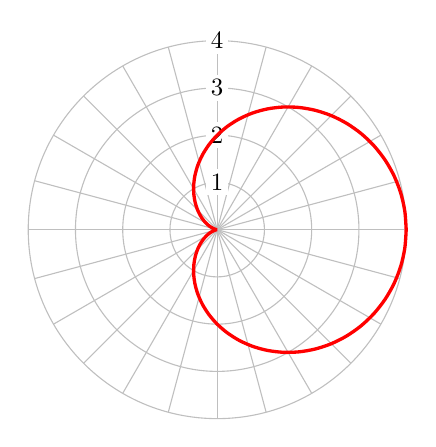
\begin{tikzpicture} [scale=.6]
\coordinate(O) at (0,0);
\foreach \angle [count=\xi] in {0, 15, ..., 345}{
  \draw[lightgray] (\angle:0) -- (\angle:4);
}
\foreach \r in {1,2,3,4} {
\draw[lightgray] (O) circle (\r);
\node[fill=white, inner sep = 2, text=black, scale=.9] at (90:\r) {$\r$};
}
\draw[domain=0:2,smooth, samples=65,variable=\x,red,very thick] plot ({180*\x)}:{2+2*cos(180*\x});
\end{tikzpicture}
\newline


hp10-2-60 cardioid

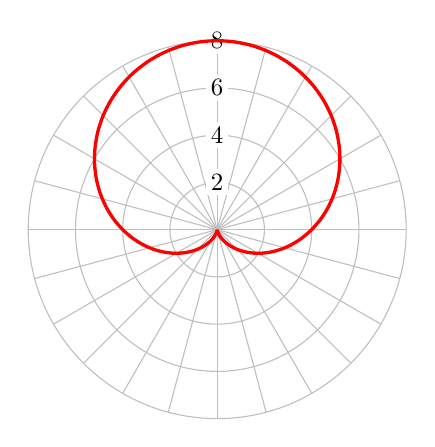
\begin{tikzpicture} [scale=.3]
\coordinate(O) at (0,0);
\foreach \angle [count=\xi] in {0, 15, ..., 345}{
  \draw[lightgray] (\angle:0) -- (\angle:8);
}
\foreach \r in {2,4,6,8} {
\draw[lightgray] (O) circle (\r);
\node[fill=white, inner sep = 2, text=black, scale=.9] at (90:\r) {$\r$};
}
\draw[domain=0:2,smooth, samples=65,variable=\x,red,very thick] plot ({180*\x)}:{4+4*sin(180*\x});
\end{tikzpicture}
\newline



hp10-2-61 five-petal rose

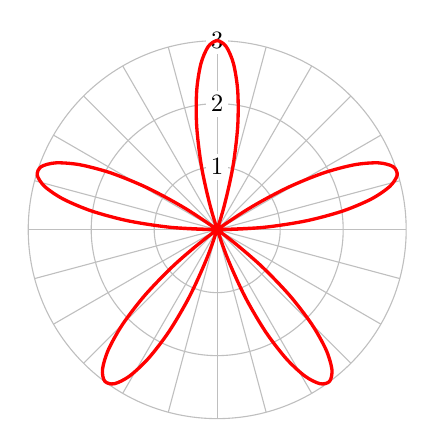
\begin{tikzpicture} [scale=0.8]
\coordinate(O) at (0,0);
\foreach \angle [count=\xi] in {0, 15, ..., 345}{
  \draw[lightgray] (\angle:0) -- (\angle:3);
}
\foreach \r in {1,2,3} {
\draw[lightgray] (O) circle (\r);
\node[fill=white, inner sep = 2, text=black, scale=.9] at (90:\r) {$\r$};
}
\draw[domain=0:2,smooth, samples=129,variable=\x,red,very thick] plot ({180*\x}:{3*sin(900*\x))});
\end{tikzpicture}
\newline



hp10-2-62 four-petal rose

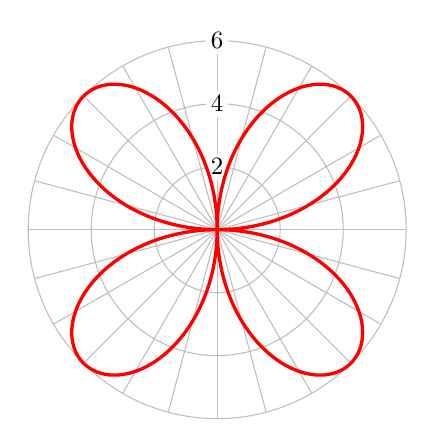
\begin{tikzpicture} [scale=0.4]
\coordinate(O) at (0,0);
\foreach \angle [count=\xi] in {0, 15, ..., 345}{
  \draw[lightgray] (\angle:0) -- (\angle:6);
}
\foreach \r in {2,4,6} {
\draw[lightgray] (O) circle (\r);
\node[fill=white, inner sep = 2, text=black, scale=.9] at (90:\r) {$\r$};
}
\draw[domain=0:2,smooth, samples=129,variable=\x,red,very thick] plot ({180*\x}:{6*sin(360*\x))});
\end{tikzpicture}
\newline


hp10-2-63 circle

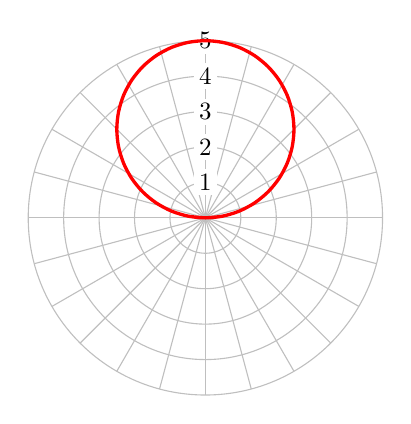
\begin{tikzpicture} [scale=.45]
\coordinate(O) at (0,0);
\foreach \angle [count=\xi] in {0, 15, ..., 345}{
  \draw[lightgray] (\angle:0) -- (\angle:5);
}
\foreach \r in {1,2,3,4,5} {
\draw[lightgray] (O) circle (\r);
\node[fill=white, inner sep = 2, text=black, scale=.9] at (90:\r) {$\r$};
}
\draw[domain=0:2,smooth, samples=65,variable=\x,red,very thick] plot ({180*\x)}:{5*sin(180*\x});
\end{tikzpicture}
\newline


hp10-2-64 circle

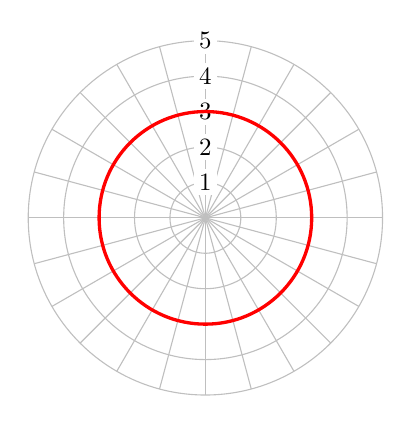
\begin{tikzpicture} [scale=.45]
\coordinate(O) at (0,0);
\foreach \angle [count=\xi] in {0, 15, ..., 345}{
  \draw[lightgray] (\angle:0) -- (\angle:5);
}
\foreach \r in {1,2,3,4,5} {
\draw[lightgray] (O) circle (\r);
\node[fill=white, inner sep = 2, text=black, scale=.9] at (90:\r) {$\r$};
}
\draw[red,very thick] (O) circle (3cm);
\end{tikzpicture}
\newline



hp10-2-65 limacon

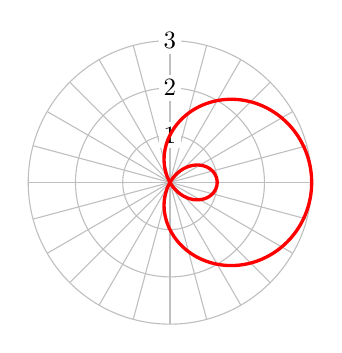
\begin{tikzpicture} [scale=0.6]
\coordinate(O) at (0,0);
\foreach \angle [count=\xi] in {0, 15, ..., 345}{
  \draw[lightgray] (\angle:0) -- (\angle:3);
}
\foreach \r in {1,2,3} {
\draw[lightgray] (O) circle (\r);
\node[fill=white, inner sep = 2, text=black, scale=.9] at (90:\r) {$\r$};
}
\draw[domain=0:2,smooth, samples=129,variable=\x,red,very thick] plot ({180*\x}:{1+2*cos(180*\x))});
\end{tikzpicture}
\newline


hp10-2-66 limacon

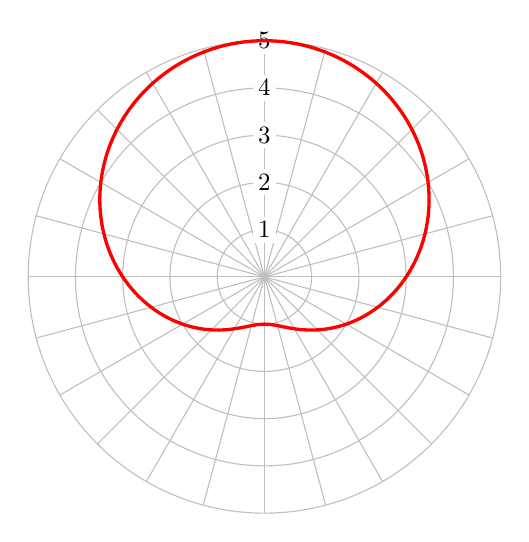
\begin{tikzpicture} [scale=.6]
\coordinate(O) at (0,0);
\foreach \angle [count=\xi] in {0, 15, ..., 345}{
  \draw[lightgray] (\angle:0) -- (\angle:5);
}
\foreach \r in {1,2,3,4,5} {
\draw[lightgray] (O) circle (\r);
\node[fill=white, inner sep = 2, text=black, scale=.9] at (90:\r) {$\r$};
}
\draw[domain=0:2,smooth, samples=129,variable=\x,red,very thick] plot ({180*\x}:{3+2*sin(180*\x))});
\end{tikzpicture}
\newline


hp10-2-77ans

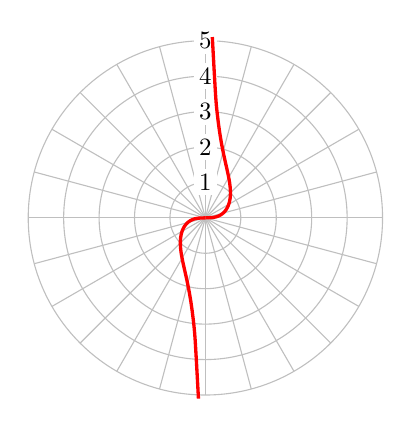
\begin{tikzpicture} [scale=.45]
\coordinate(O) at (0,0);
\foreach \angle [count=\xi] in {0, 15, ..., 345}{
  \draw[lightgray] (\angle:0) -- (\angle:5);
}
\foreach \r in {1,2,3,4,5} {
\draw[lightgray] (O) circle (\r);
\node[fill=white, inner sep = 2, text=black, scale=.9] at (90:\r) {$\r$};
}
\draw[domain=0:.488,smooth, samples=33,variable=\x,red,very thick] plot ({180*\x}:{sqrt(tan(180*\x)))});
\draw[domain=0:.488,smooth, samples=33,variable=\x,red,very thick] plot ({180*\x}:{-sqrt(tan(180*\x)))});
\end{tikzpicture}
\newline


hp10-2-79ans conchoid

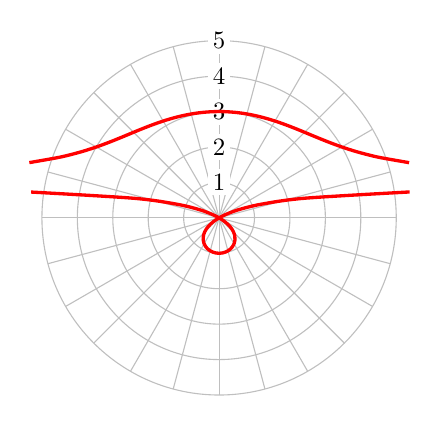
\begin{tikzpicture} [scale=.45]
\coordinate(O) at (0,0);
\foreach \angle [count=\xi] in {0, 15, ..., 345}{
  \draw[lightgray] (\angle:0) -- (\angle:5);
}
\foreach \r in {1,2,3,4,5} {
\draw[lightgray] (O) circle (\r);
\node[fill=white, inner sep = 2, text=black, scale=.9] at (90:\r) {$\r$};
}
\draw[domain=.043:.957,smooth, samples=33,variable=\x,red,very thick] plot ({180*\x}:{1/sin(180*\x)-2});
\draw[domain=1.09:1.91,smooth, samples=33,variable=\x,red,very thick] plot ({180*\x}:{1/sin(180*\x)-2});
\end{tikzpicture}
\newline


hp10-2-79ans strophoid

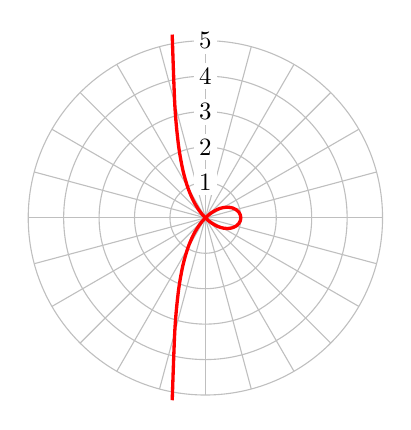
\begin{tikzpicture} [scale=.45]
\coordinate(O) at (0,0);
\foreach \angle [count=\xi] in {0, 15, ..., 345}{
  \draw[lightgray] (\angle:0) -- (\angle:5);
}
\foreach \r in {1,2,3,4,5} {
\draw[lightgray] (O) circle (\r);
\node[fill=white, inner sep = 2, text=black, scale=.9] at (90:\r) {$\r$};
}
\draw[domain=-.443:.443,smooth, samples=33,variable=\x,red,very thick] plot ({180*\x}:{cos(360*\x)/cos(180*\x)});
\end{tikzpicture}
\newline


hp10-2-81ans ?spiral?

\begin{tikzpicture} [scale=.45]
\coordinate(O) at (0,0);
\foreach \angle [count=\xi] in {0, 15, ..., 345}{
  \draw[lightgray] (\angle:0) -- (\angle:5);
}
\foreach \r in {1,2,3,4,5} {
\draw[lightgray] (O) circle (\r);
\node[fill=white, inner sep = 2, text=black, scale=.9] at (90:\r) {$\r$};
}
\draw[domain=.0129:6,smooth, samples=257,variable=\x,red,very thick] plot ({180*\x}:{1/sqrt(pi*\x)});
\end{tikzpicture}
\newline






\end{document}
